\documentclass[titlepage]{article}

\usepackage{listings}
\usepackage[dvipsnames,table]{xcolor}
\usepackage[firstpage]{draftwatermark}
\usepackage{eso-pic}
\usepackage[T1]{fontenc}
\usepackage[french]{babel}
\usepackage[utf8]{inputenc}
\usepackage[hidelinks]{hyperref}
% \usepackage[hyperpageref]{backref}
% \usepackage{chngcntr}
\usepackage{amsmath}
\usepackage{amssymb}
\usepackage{geometry} % Règle la marge en haut/bas/droite/gauche
\usepackage{times} % Change la police en Times new roman
\usepackage{etoolbox}
\usepackage{titlesec}
\usepackage{tocloft}
\usepackage{multirow}
\usepackage{tikz} % Pour faire des figures 3D
\usepackage{subcaption}

\SetWatermarkLightness{0.8}
\SetWatermarkAngle{50}
\SetWatermarkScale{1.4}
\SetWatermarkFontSize{3cm}
\SetWatermarkText{Confidentiel}

\usetikzlibrary{patterns,perspective}
\usetikzlibrary{decorations.pathreplacing,calligraphy}

% --- Permet de régler l'espace entre le nombre et le titre dans toc ---

\setlength\cftsubsecnumwidth{1em}
\setlength\cftsubsubsecnumwidth{1.8em}
\setlength\cftparanumwidth{2.6em}

\setlength\cftsubsubsecindent{2.6em}
\setlength\cftparaindent{4.4em}

\setlength\cftfignumwidth{2.8em}

% --- Changement nombre figure --- (package chngcntr)

\counterwithin{figure}{section}

% --- Réglages du package french pour que les tirets soient des points dans les listes ---

%\frenchbsetup{StandardLists=true}

% --- Règle les marges ---

\geometry{hmargin=2.5cm,vmargin=2.5cm}

% --- glossary ---

\usepackage[toc,acronym]{glossaries}
\makeglossaries

% --- Nomenclature ---

\usepackage{nomencl}
\makenomenclature

\renewcommand\nomgroup[1]{%
  \item[\bfseries
  \ifstrequal{#1}{A}{Lettres latines}{%
  \ifstrequal{#1}{B}{Lettres grecques}{%
  \ifstrequal{#1}{C}{Indices}{%
  \ifstrequal{#1}{D}{Exposants}{%
  \ifstrequal{#1}{E}{Nombres sans dimension}{}}}}}%
]}

\newcommand{\nomunit}[1]{%
\renewcommand{\nomentryend}{\hspace*{\fill}#1}}

% --- Pour mettre les logos de l'ISIMA et A&D sur la page titre ---
 
\newcommand{\HRule}{\rule{\linewidth}{0.5mm}}
\newcommand{\blap}[1]{\vbox to 0pt{#1\vss}}
\newcommand\AtUpperLeftCorner[3]{%
  \put(\LenToUnit{#1},\LenToUnit{\dimexpr\paperheight-#2}){\blap{#3}}%
}
\newcommand\AtUpperRightCorner[3]{%
  \put(\LenToUnit{\dimexpr\paperwidth-#1},\LenToUnit{\dimexpr\paperheight-#2}){\blap{\llap{#3}}}%
}

% --- Section et autres ---

\setcounter{tocdepth}{4}
\setcounter{secnumdepth}{4}

\newcommand{\wsection}[1]{
\section*{#1}
\addcontentsline{toc}{section}{#1}
}
\newcommand{\wsubsection}[1]{
\subsection*{#1}
\addcontentsline{toc}{subsection}{#1}
}

\titleformat*{\section}{\huge\bfseries}
\titleformat*{\subsection}{\LARGE\bfseries}
\titleformat*{\subsubsection}{\Large\bfseries}
\titleformat*{\paragraph}{\large\bfseries}
\titleformat*{\subparagraph}{\large\bfseries}

\renewcommand{\thesection}{\Roman{section}}
\renewcommand{\thesubsection}{\arabic{subsection}}
\renewcommand{\thesubsubsection}{\arabic{subsection}.\arabic{subsubsection}}
\renewcommand{\theparagraph}{\arabic{subsection}.\arabic{subsubsection}.\arabic{paragraph}}

% --- ref ---

\newcommand{\completeref}[1]{\autoref{#1}, page \pageref{#1}}
\newcommand{\bracompref}[1]{\autoref{#1} (page \pageref{#1})}

\newcommand{\Iref}[1]{\cRM{1}.\ref{#1}}
\newcommand{\IIref}[1]{\cRM{2}.\ref{#1}}
\newcommand{\IIIref}[1]{\cRM{3}.\ref{#1}}

% --- forge ---

\newcommand{\forge}{FORGE$^\circledR$}
\newcommand{\forgews}{FORGE$^\circledR$ }

% --- chiffre romains ---

% Romain
\newcommand{\cRM}[1]{\MakeUppercase{\romannumeral #1}} % Capital
\newcommand{\cRm}[1]{\textsc{\romannumeral #1}} % Petit majuscule
\newcommand{\crm}[1]{\romannumeral #1}
% Siècle %
\newcommand{\siecle}[1]{\cRM{#1}\textsuperscript{e}~siècle}

% --- listings ---

\definecolor{codegreen}{rgb}{0,0.6,0}
\definecolor{codegray}{rgb}{0.5,0.5,0.5}
\definecolor{codepurple}{rgb}{0.58,0,0.82}
\definecolor{backcolour}{rgb}{0.95,0.95,0.92}

\lstdefinestyle{mystyle}{
    backgroundcolor=\color{backcolour},   
    commentstyle=\color{codegreen},
    keywordstyle=\color{magenta},
    numberstyle=\tiny\color{codegray},
    stringstyle=\color{codepurple},
    basicstyle=\ttfamily\footnotesize,
    breakatwhitespace=false,         
    breaklines=true,                 
    captionpos=b,                    
    keepspaces=true,                 
    numbers=left,                    
    numbersep=5pt,                  
    showspaces=false,                
    showstringspaces=false,
    showtabs=false,                  
    tabsize=2
}

\definecolor{classclr}{RGB}{71,196,160}
\definecolor{funcclr}{RGB}{255,219,87}

\newcommand{\class}[1]{\textcolor{Emerald}{#1}}
\newcommand{\widget}[1]{\textcolor{OrangeRed}{#1}}
\newcommand{\function}[1]{\textcolor{Orange}{#1}}
\newcommand{\variable}[1]{\textcolor{Cyan}{#1}}

\lstset{style=mystyle}

\renewcommand\lstlistingname{\'{E}lément de code}
\renewcommand\lstlistlistingname{Table des éléments de code}
\def\lstlistingautorefname{élément de code}

\newacronym{epun}{EPUN}{\'{E}cole Polytechnique de l'Université de Nantes}

\title{\Huge{Titre}}
\author{Rapport d'élève ingénieur\\
Alternance de $3^{\text{ème}}$ année\\
Filière F4 : Modélisation mathématique et science des données\\
Présenté par : Louis \textsc{Encinas}\\\\
Tuteur ISIMA : Renaud \textsc{Chicoisne}\\
Tuteur entreprise : Sébastien \textsc{Andre}\\\\\\\\
Date soutenance : ??\\
Durée du stage : ??}
\date{\today}

\begin{document}

\begin{titlepage}
\AddToShipoutPicture*{
        \AtUpperLeftCorner{1.5cm}{1cm}{\includegraphics[width=8cm]{image/isima.png}}
        \AtUpperRightCorner{1.5cm}{1cm}{\includegraphics[width=8cm]{image/A&D.jpg}}
    }
\maketitle
\end{titlepage}

\shipout\null

\pagenumbering{roman}

\input{sections/remerciement}
\newpage

\wsection{Résumé}

\noindent \textbf{Mots-clés} :

\wsection{Abstract}

\noindent \textbf{Key-words} :
\newpage

\tableofcontents
\addcontentsline{toc}{section}{Table des matières}
\newpage

\listoffigures
\addcontentsline{toc}{section}{Table des figures}

\lstlistoflistings
\addcontentsline{toc}{section}{Table des éléments de code}
\newpage

\pagenumbering{arabic}

\wsection{Introduction de l'étude}
\newpage

\section{Partie 1 \label{sec:partie_1}}

\subsection{Partie 1.1} % On peut aussi mettre le label juste en dessous
\label{sec:partie_1_1}

\subsubsection{Partie 1.1.1}

\autoref{fig:chat1}

\begin{figure}[ht]
	\centering
	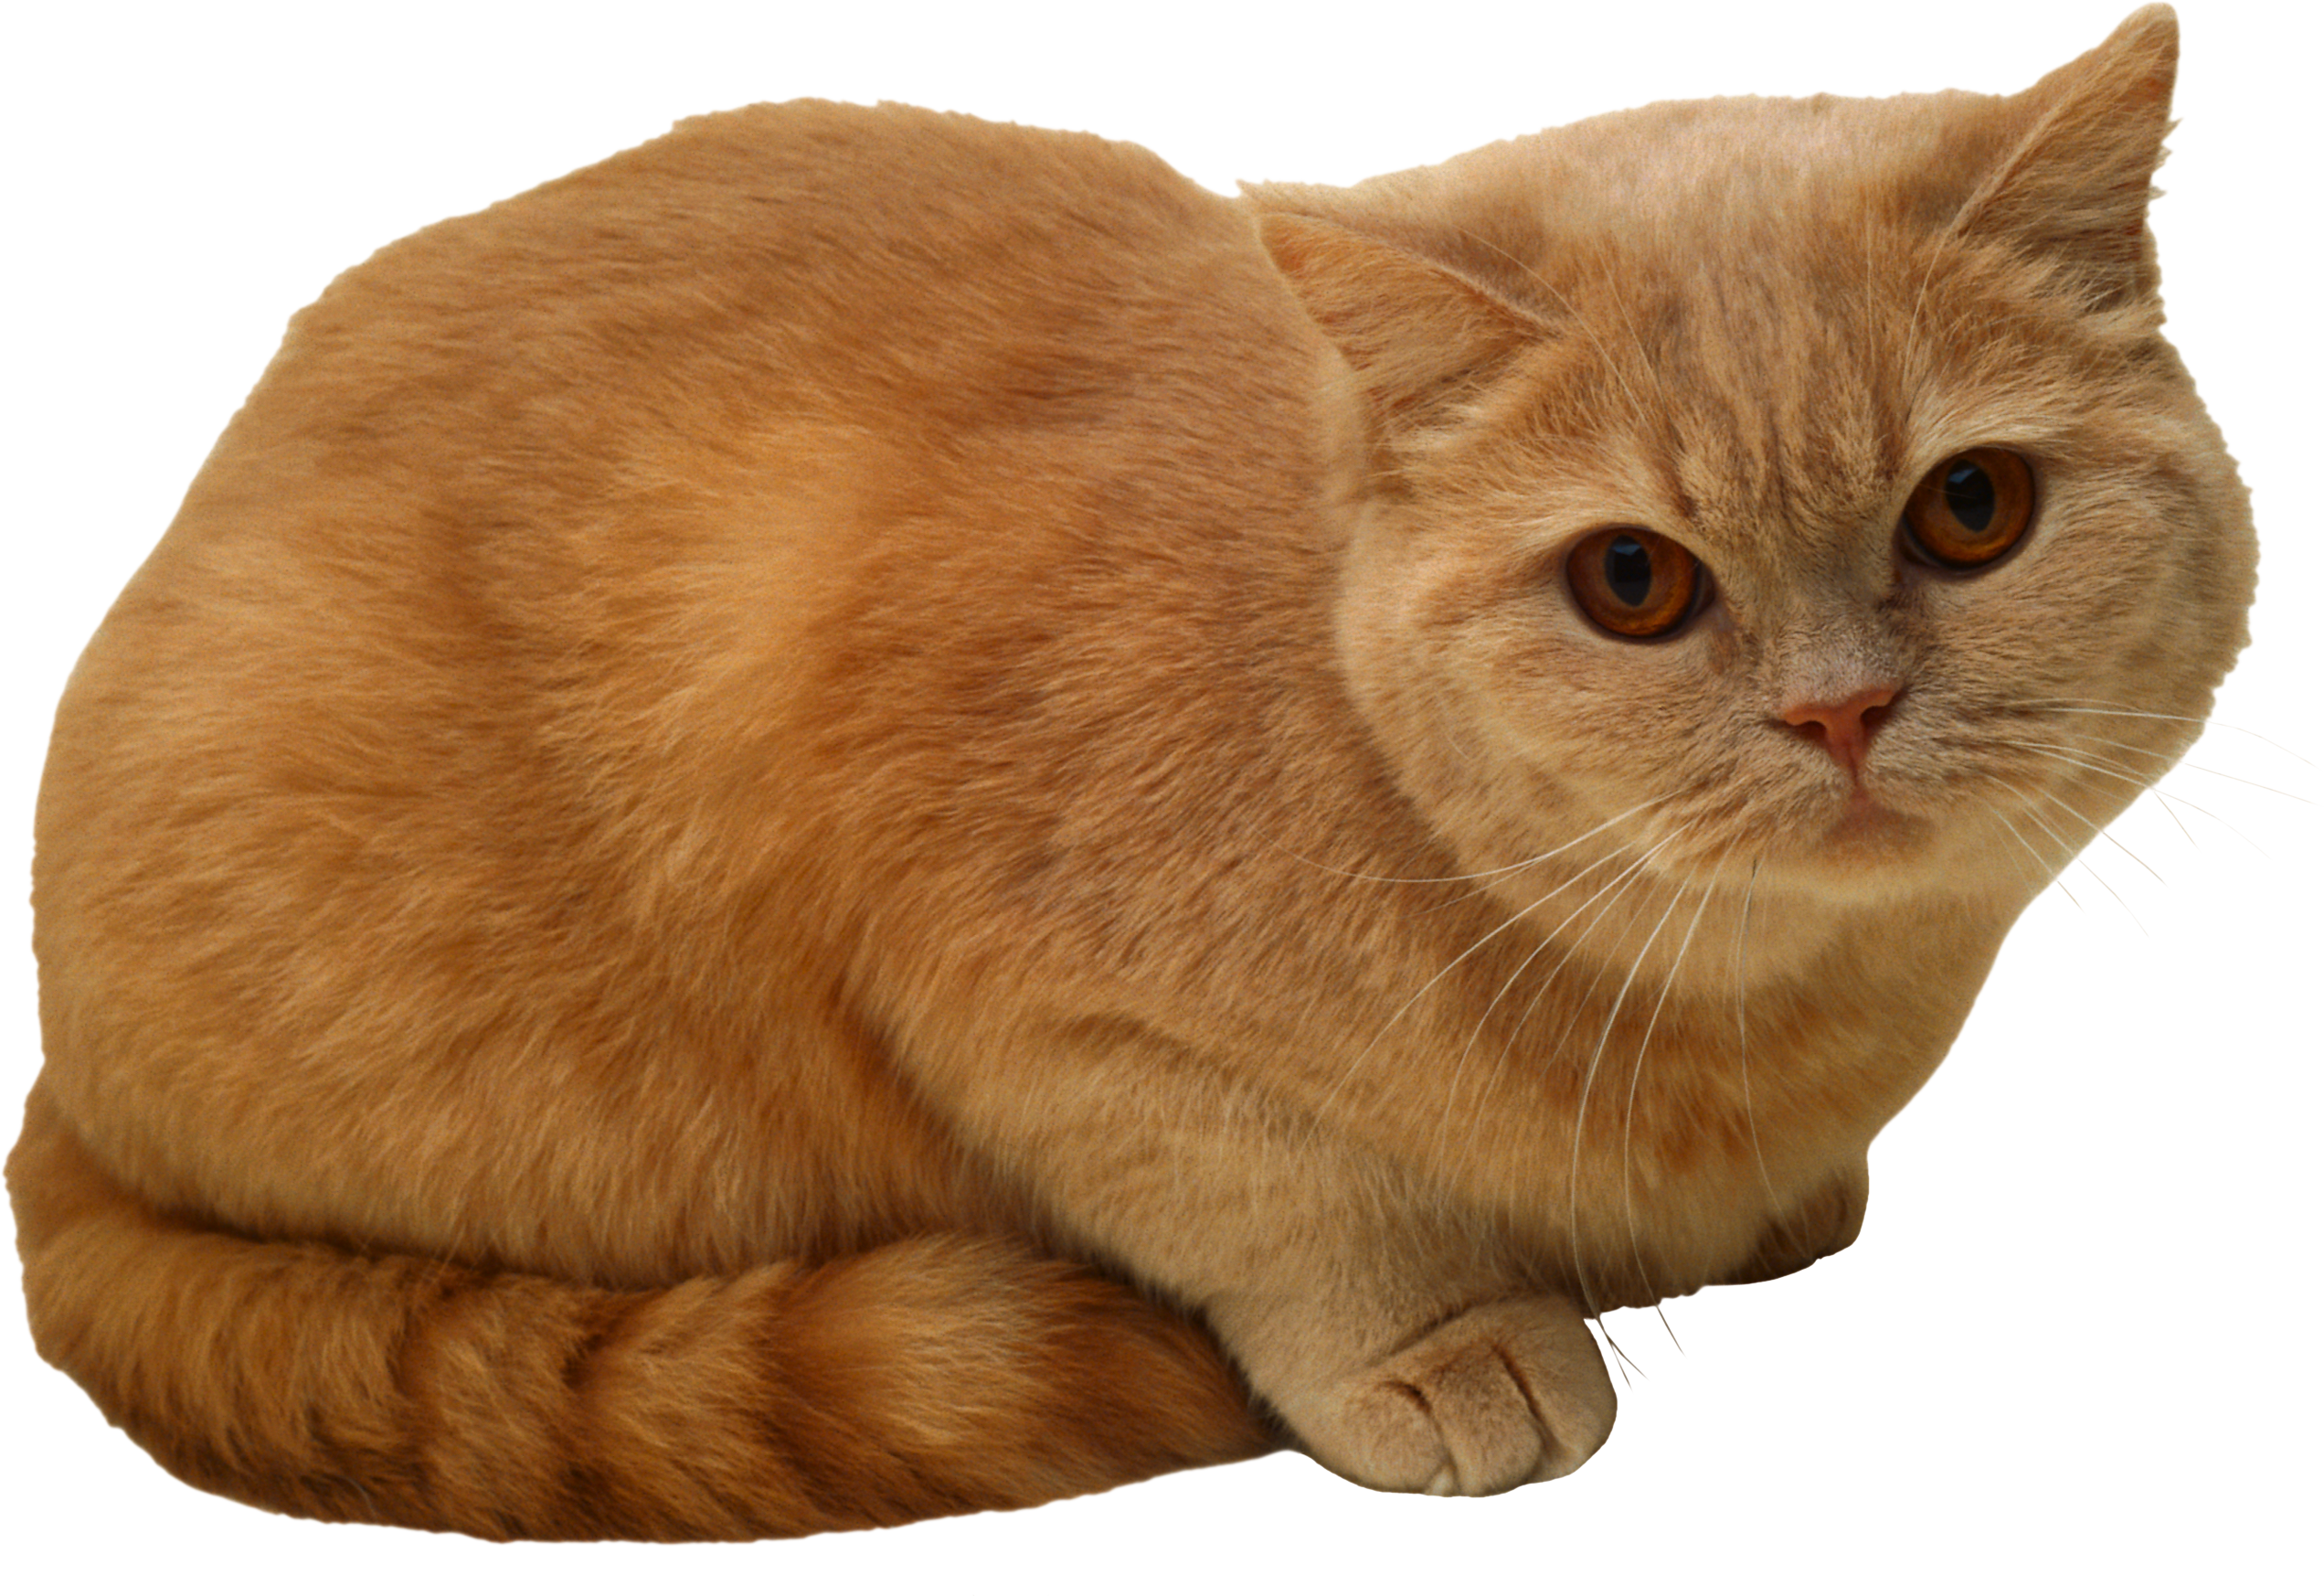
\includegraphics[width=.9\linewidth]{image/chat.png}
	\caption{Représentation d'un chat}
	\label{fig:chat1}
\end{figure}

\subsubsection{Partie 1.1.2}

\subparagraph{Partie 1.1.2.1}
~~\newline

\subparagraph{Partie 1.1.2.2}
~~\newline


\subsubsection{Partie 1.1.3 \label{sec:partie_1_1_3}}

\completeref{fig:chat3}

\bracompref{fig:chat3}

\begin{figure}[ht]
	\centering
	\begin{subfigure}[c]{0.45\textwidth}
		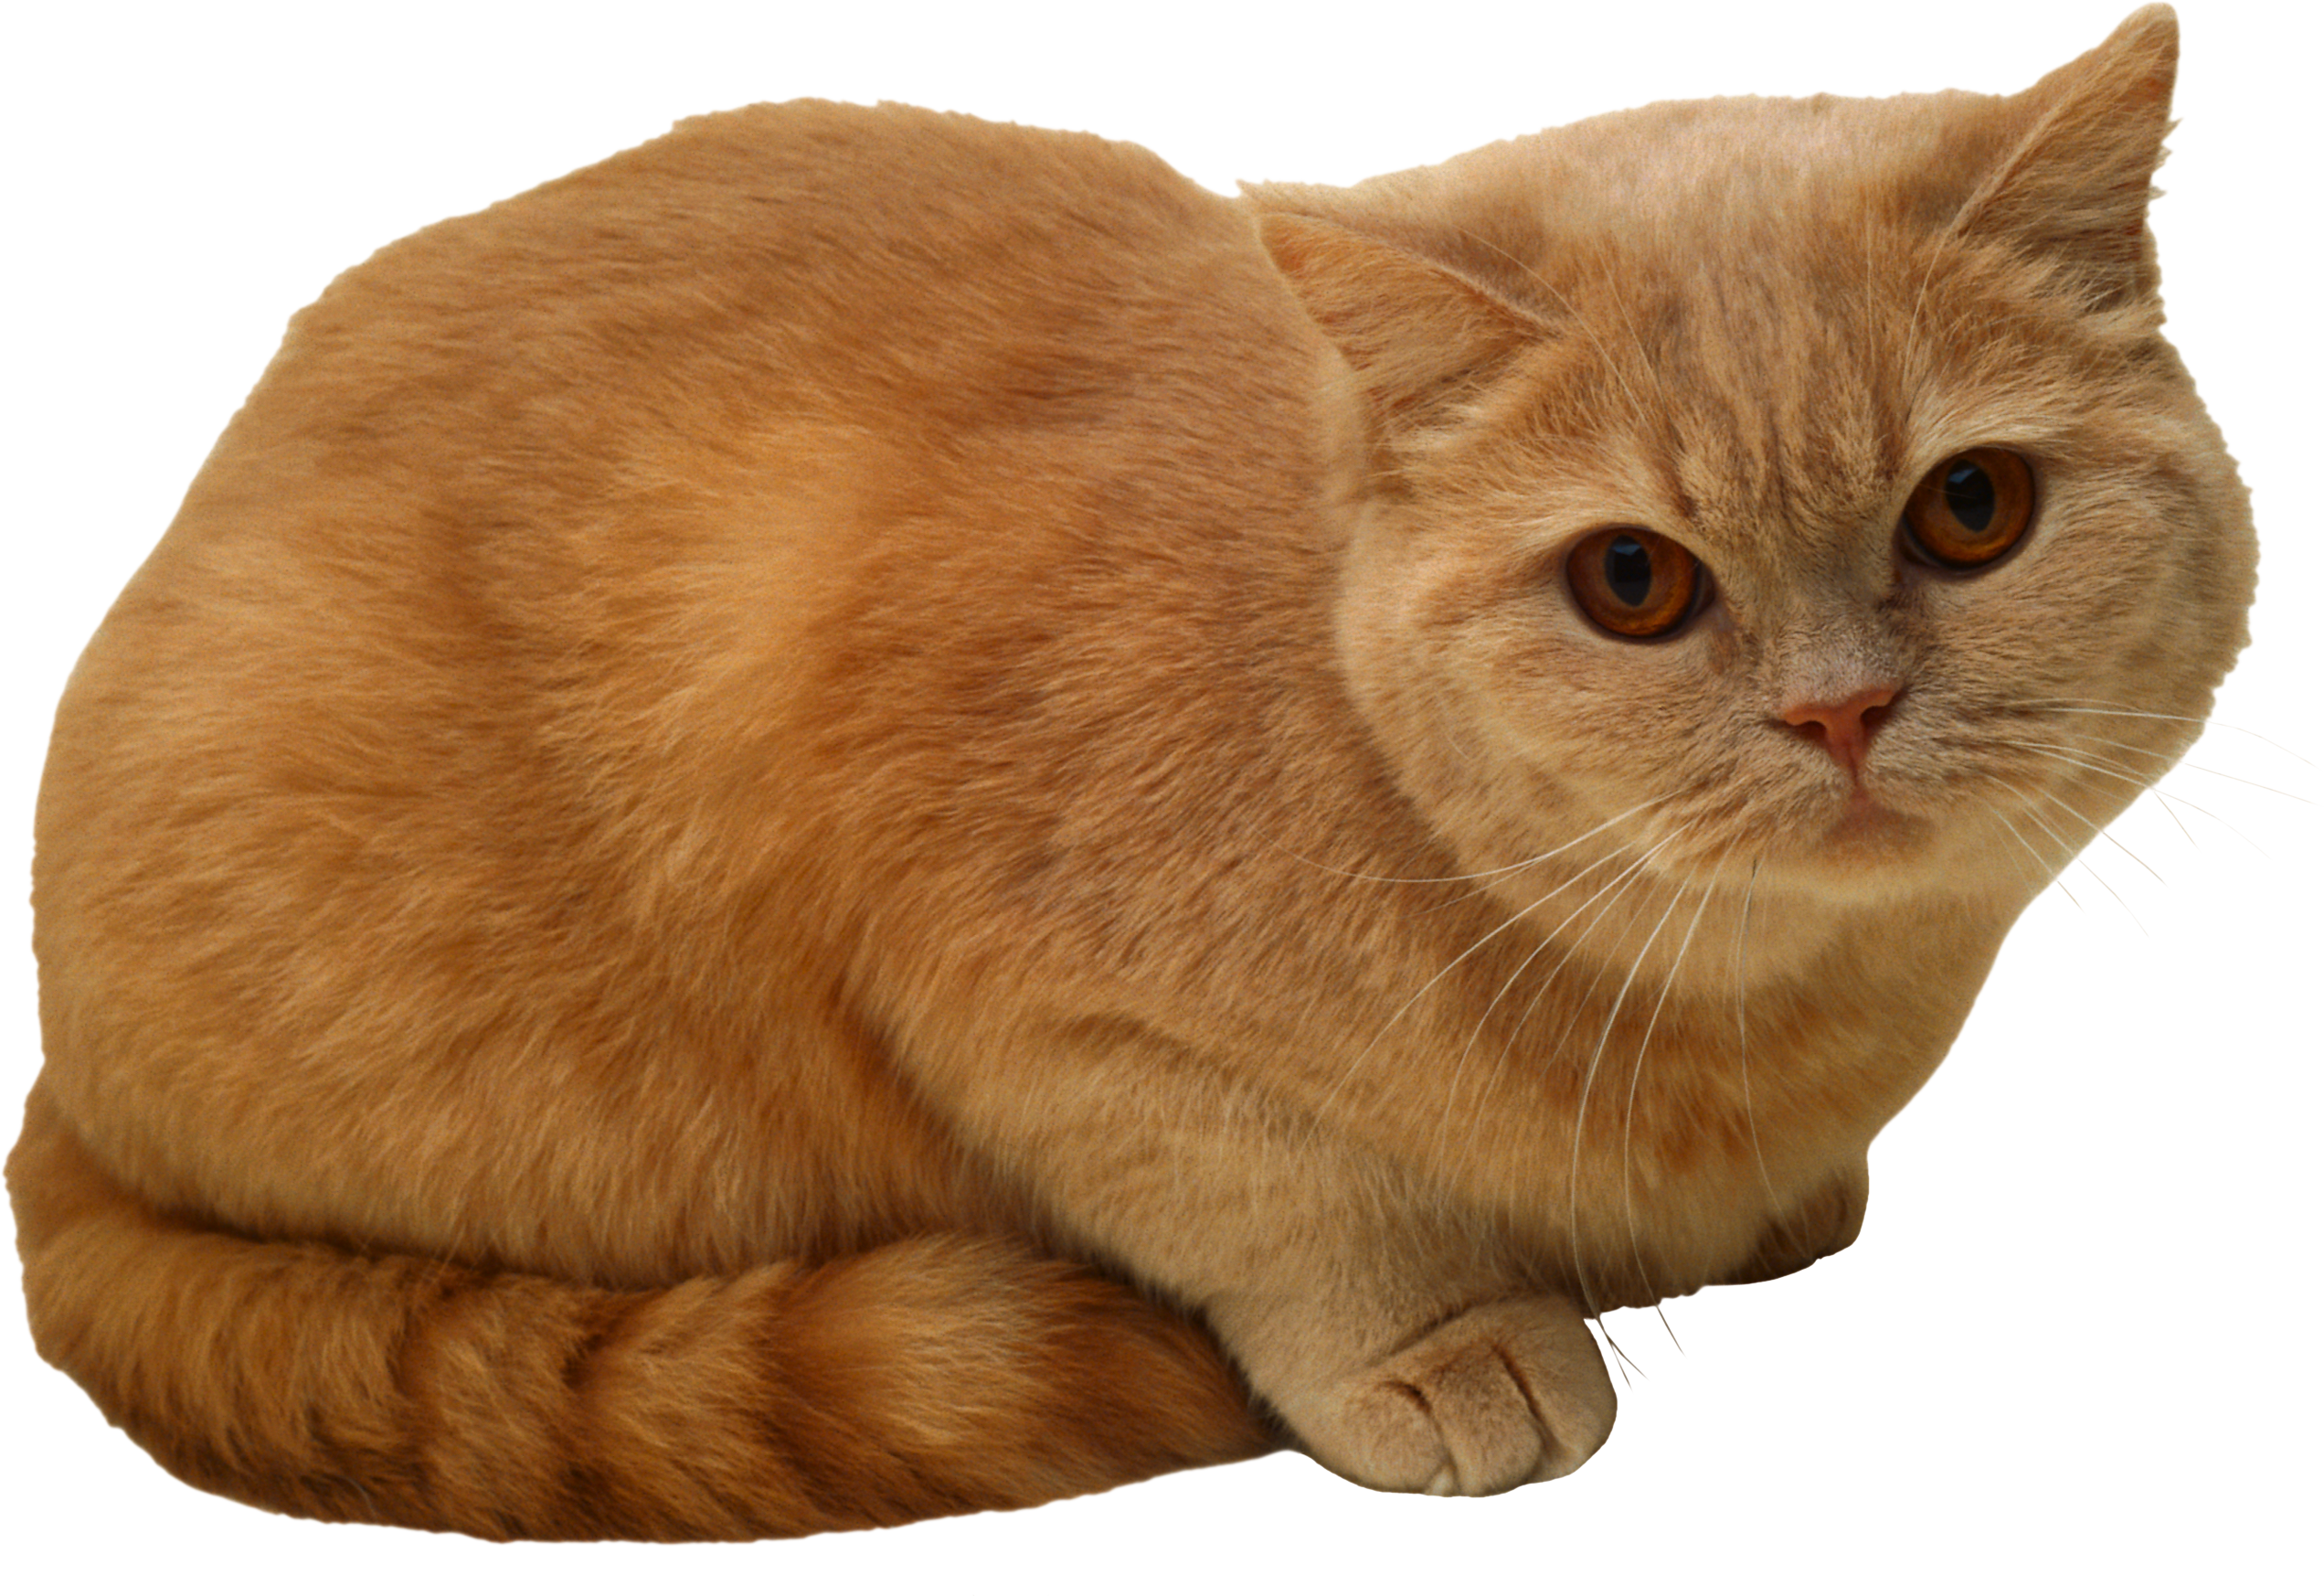
\includegraphics[width=\textwidth]{image/chat.png}
		\caption{Chat gauche}
	\end{subfigure}
	\hfill
	\begin{subfigure}[c]{0.45\textwidth}
		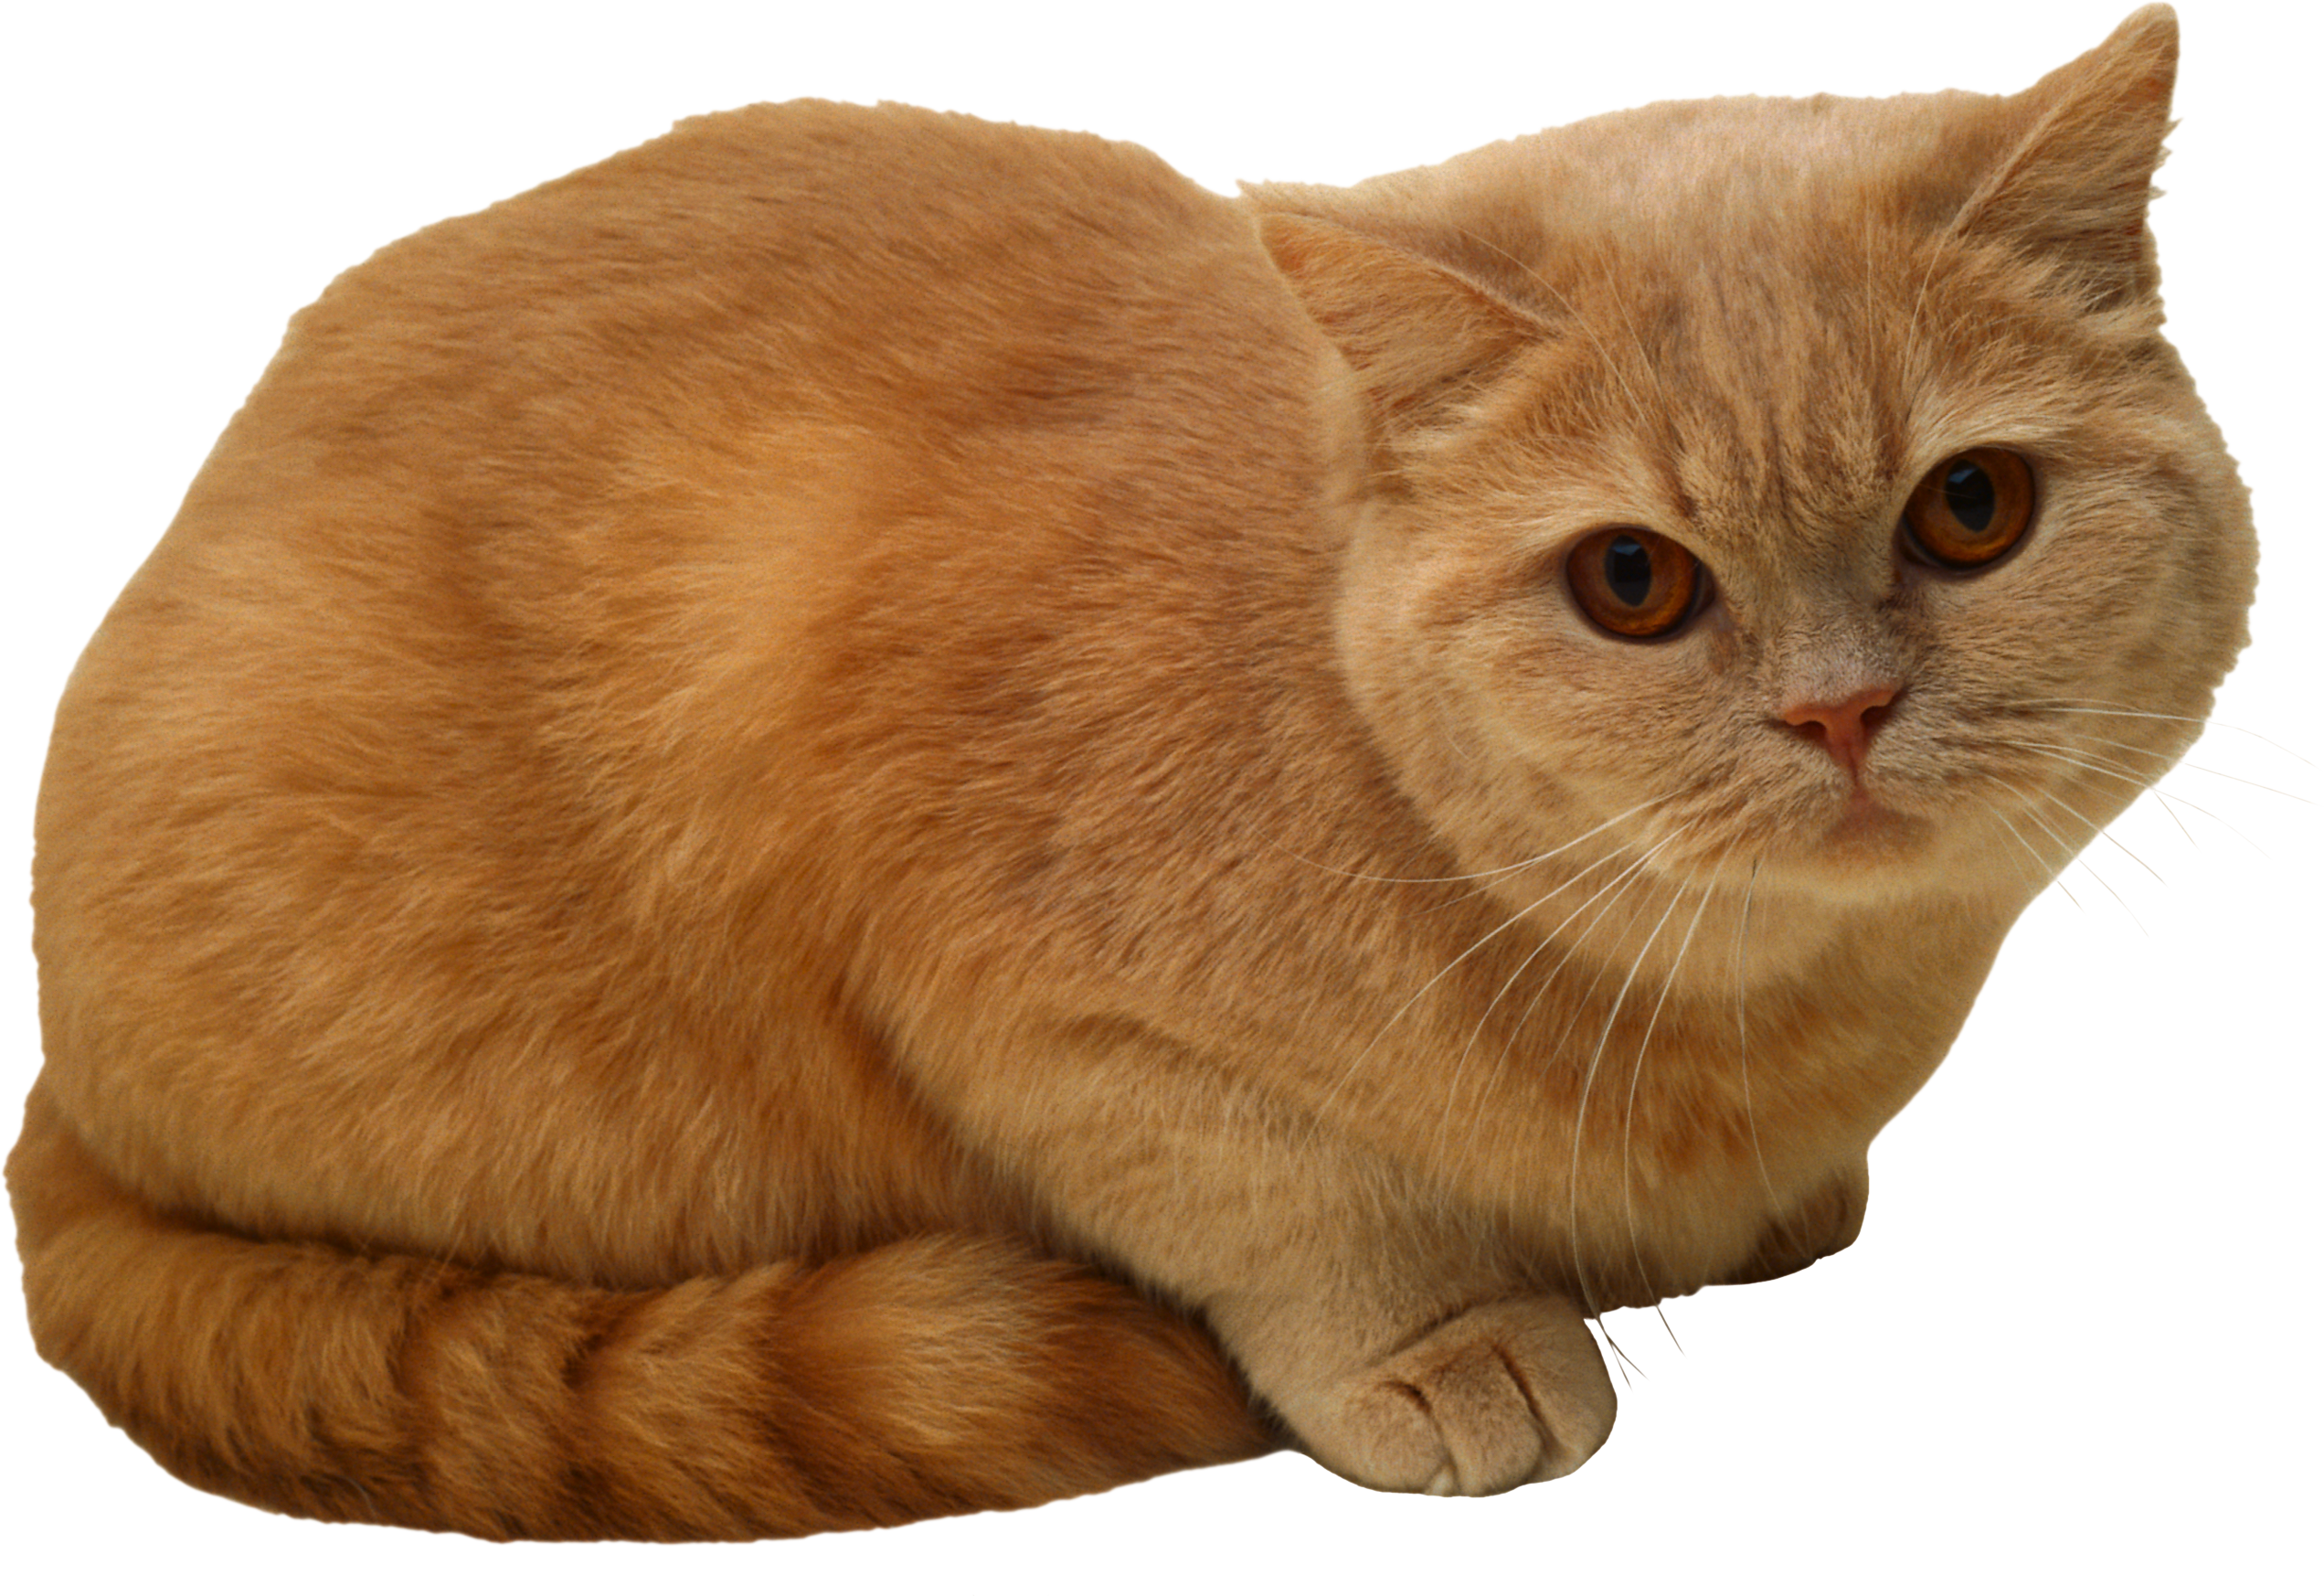
\includegraphics[width=\textwidth]{image/chat.png}
		\caption{Chat droite}
	\end{subfigure}
			
	\caption{Deux chats}
	\label{fig:chat3}
\end{figure}

\paragraph{Partie 1.1.3.1 \label{sec:partie_1_1_3_1}}
~~\newline

\paragraph{Partie 1.1.3.2}
\label{sec:partie_1_1_3_2}
~~\newline

Lien vers un titre : \Iref{sec:partie_1_1}

\subparagraph{Partie 1.1.3.2.1}
~~\newline

Acronyme full : \acrfull{epun}; Acronyme long : \acrlong{epun}; Acronyme short : \acrshort{epun}\newline

Note de bas de page\footnote{Note de base de page}\newline

Citation bibli : \cite{scikit-learn}, \cite{gnikit2022}, \cite{gnikit2022,scikit-learn}\newline

\begin{equation}
	y = f(\beta,X) + \varepsilon
	\label{eq:model}
\end{equation}

Lien vers l'équation : \ref{eq:model}

% Important : il ne faut pas que un code soit divisé entre deux page sinon il y a une erreur à la compile

\newpage
\autoref{el:vehicule}
\begin{lstlisting}[language=Python, caption=Définition de classe en Python, label=el:vehicule]
    class Vehicule:

        def __init__(self, marque, annee):
            self.marque = marque
            self.annee = annee

        def avancer(self):
            ...
\end{lstlisting}
\newpage

\section{Partie 2}
\label{sec:partie_2}

\subsection{Partie 2.1}
\label{sec:partie_2_1}

\subsection{Partie 2.2}
\label{sec:partie_2_2}
\newpage

\section{Partie 3}

\subsection{Partie 3.1}

\subsection{Partie 3.2}
\newpage

\input{sections/conclusion}
\newpage

\pagenumbering{Roman}
\bibliographystyle{abbrv}
\bibliography{bibliography}
\addcontentsline{toc}{section}{Références}
\newpage

\printglossaries

\nomenclature[A]{$h$}{coefficient d'échange thermique \nomunit{W.m$^{-2}$.K$^{-1}$}}

\nomenclature[B]{$\beta$}{vecteur des coefficients d'un modèle de régression}

\nomenclature[C]{$max$}{maximum}

\printnomenclature
\addcontentsline{toc}{section}{Nomenclature}
\newpage

\input{sections/annexe.tex}
\addcontentsline{toc}{section}{Annexe}

\end{document}